\documentclass{article}
\usepackage{amsmath}
\usepackage{graphicx}
\begin{document}
\section{Lists}
\begin{itemize}
  \item First item
  \item Second item with \textbf{bold}
  \item Third item
\end{itemize}

\begin{enumerate}
  \item Numbered one
  \item Numbered two
\end{enumerate}

\section{Figure}
\begin{figure}[h]
  \centering
  \fbox{Placeholder image}
  \caption{Sample figure}
  \label{fig:sample}
\end{figure}

\section{Table}
\begin{table}[h]
  \centering
  \begin{tabular}{lcc}
    \toprule
    Name & Value & Unit \\
    \midrule
    Alpha & 1.23 & m \\
    Beta & 4.56 & s \\
    \bottomrule
  \end{tabular}
  \caption{Sample table}
  \label{tab:sample}
\end{table}

\section{TikZ}
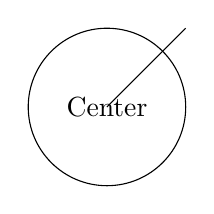
\begin{tikzpicture}
  \draw (0,0) circle (1);
  \draw (0,0) -- (1,1);
  \node at (0,0) {Center};
\end{tikzpicture}

\section{Deep Nesting}
\begin{itemize}
  \item Level 1
  \begin{itemize}
    \item Level 2
    \begin{itemize}
      \item Level 3
    \end{itemize}
  \end{itemize}
\end{itemize}

\section{Empty Environments}
\begin{equation}
\end{equation}

\begin{itemize}
\end{itemize}

\section{Unknown Environment}
\begin{myenv}
  Content in unknown env.
\end{myenv}

\begin{customblock}{title}
  Some content.
\end{customblock}

\section{Nested Math}
\begin{equation}
  \begin{cases}
    \begin{pmatrix}
    a               & b \\
    c               & d
    \end{pmatrix}   & \text{if } n = 1 \\
    \begin{pmatrix}
    e               & f \\
    g               & h
    \end{pmatrix}   & \text{if } n = 2
  \end{cases}
\end{equation}
\end{document}